% Requires (already in main.tex): \usepackage{tikz}, \usetikzlibrary{arrows.meta,positioning}
% Toy example: what the LLM hands back. Place right after the "LLM writes rules, not edits" frame.

\begin{frame}{Edit vs.\ rule: the same saving, on a toy circuit}

\centering
\resizebox{0.80\textwidth}{!}{%
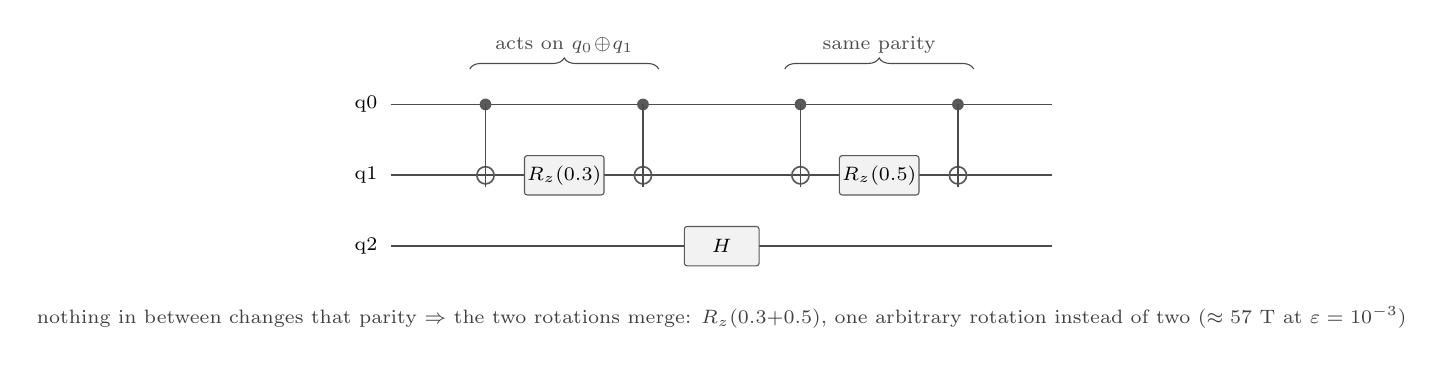
\begin{tikzpicture}[x=1cm, y=1cm,
    wire/.style={line width=0.6pt, gray!60!black},
    gate/.style={draw=gray!70!black, fill=gray!10, rounded corners=1pt,
                 minimum width=0.95cm, minimum height=0.5cm, font=\scriptsize, inner sep=1pt},
    ctrl/.style={circle, fill=gray!70!black, inner sep=1.5pt},
    targ/.style={circle, draw=gray!70!black, line width=0.6pt, inner sep=2.2pt}]

  \foreach \y/\lab in {0/q0, -0.9/q1, -1.8/q2} {
    \draw[wire] (-0.2,\y) -- (8.2,\y);
    \node[left, font=\scriptsize] at (-0.25,\y) {\lab};
  }
  % cx pairs: control q0, target q1
  \foreach \x in {1,3,5,7} {
    \node[ctrl] (c\x) at (\x,0) {};
    \node[targ] (t\x) at (\x,-0.9) {};
    \draw[wire] (\x,0) -- (\x,-0.9);
    \draw[wire] (\x,-1.05) -- (\x,-0.75);
  }
  \node[gate] at (2,-0.9) {$R_z(0.3)$};
  \node[gate] at (6,-0.9) {$R_z(0.5)$};
  \node[gate] at (4,-1.8) {$H$};

  \draw[decorate, decoration={brace, amplitude=4pt}, gray!60!black]
        (0.8,0.45) -- (3.2,0.45) node[midway, above, font=\scriptsize, yshift=2pt] {acts on $q_0\!\oplus\!q_1$};
  \draw[decorate, decoration={brace, amplitude=4pt}, gray!60!black]
        (4.8,0.45) -- (7.2,0.45) node[midway, above, font=\scriptsize, yshift=2pt] {same parity};
  \node[font=\scriptsize, text=gray!50!black, align=center] at (4,-2.7)
       {nothing in between changes that parity $\Rightarrow$ the two rotations merge: $R_z(0.3{+}0.5)$,
        one arbitrary rotation instead of two ($\approx 57$ T at $\varepsilon=10^{-3}$)};
\end{tikzpicture}%
}

\vspace{0.25cm}

\begin{columns}[T]
\begin{column}{0.48\textwidth}
{\footnotesize\textbf{Before} --- the LLM typed the \alert{answer}:}
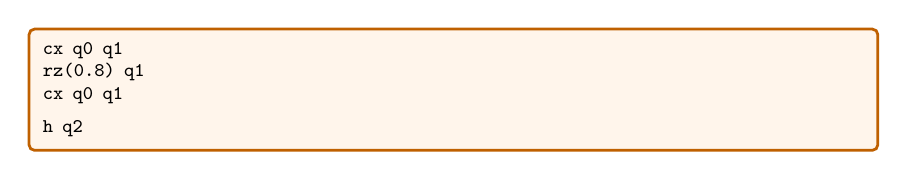
\begin{tikzpicture}
  \node[draw=orange!75!black, fill=orange!8, rounded corners=2pt, line width=1pt,
        align=left, inner sep=5pt, text width=0.86\columnwidth]
  {\ttfamily\scriptsize
   cx q0 q1\\ rz(0.8) q1\\ cx q0 q1\\ h q2};
\end{tikzpicture}
{\scriptsize
\begin{itemize}\setlength\itemsep{1pt}
  \item names \texttt{q0}, \texttt{q1}, \texttt{0.8}: true \emph{here} only
  \item same pattern 400 ops later $\to$ another LLM call
  \item carried forward only as prose hints
\end{itemize}}
\end{column}
\begin{column}{0.48\textwidth}
{\footnotesize\textbf{Now} --- the LLM types the \alert{finder}:}
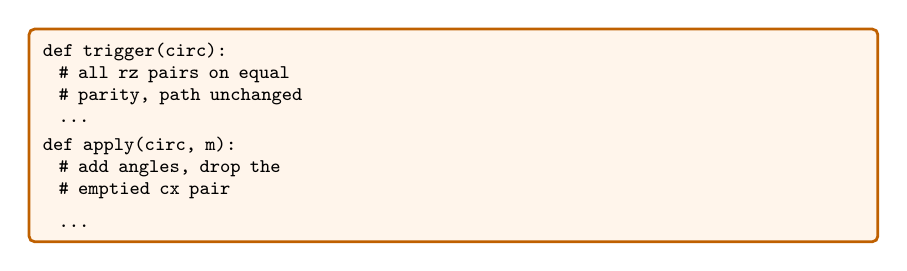
\begin{tikzpicture}
  \node[draw=orange!75!black, fill=orange!8, rounded corners=2pt, line width=1pt,
        align=left, inner sep=5pt, text width=0.86\columnwidth]
  {\ttfamily\scriptsize
   def trigger(circ):\\
   \hspace*{2mm}\# all rz pairs on equal\\
   \hspace*{2mm}\# parity, path unchanged\\
   \hspace*{2mm}...\\[2pt]
   def apply(circ, m):\\
   \hspace*{2mm}\# add angles, drop the\\
   \hspace*{2mm}\# emptied cx pair\\
   \hspace*{2mm}...};
\end{tikzpicture}
{\scriptsize
\begin{itemize}\setlength\itemsep{1pt}
  \item no qubit, no angle hard-coded
  \item code applies it to \emph{every} match, every circuit
  \item verified per application; then 0 LLM calls
\end{itemize}}
\end{column}
\end{columns}

\end{frame}
